% Global Variables
\def \titletext {Asst 02: Spooky Searching Results}
\def \creator {Shivan Modha and Ryan Mao}
\def \builddate {February 08, 2018}
\def \class {01:198:214:01}

\documentclass{article}

% Packages
\usepackage[letterpaper, portrait]{geometry}
% Configure page margins with geometry
\geometry{left=0.5in, top=0.5in, right=0.5in, bottom=0.5in, headsep=0.2cm, footskip=0.2cm}
\usepackage{amsfonts}
\usepackage{enumerate}
\usepackage{amsmath}
\usepackage{tocloft}
\usepackage[english]{babel}
%\usepackage[utf8]{inputenc}
\usepackage{fancyhdr}
\usepackage{amssymb}
%\usepackage{gensymb}
\usepackage{microtype}
\usepackage{graphicx}
\usepackage{caption}
\usepackage{subcaption}
\usepackage{tikz}
\usepackage[makeroom]{cancel}
\usepackage[]{units}

\usepackage{amsthm}
\usepackage{enumitem}

\usepackage{latexsym,ifthen,url,rotating}

\usepackage{color}
\usepackage[md]{titlesec}
\usepackage{float}
\usepackage{csquotes}

%\usepackage{showframe}
\graphicspath{ {images/} }

% Configure Header
\pagestyle{fancy}
\fancyhf{}
\lhead{\creator}
\chead{\class}
\rhead{\today}
\rfoot{\thepage}

% --- -----------------------------------------------------------------
% --- Document-specific definitions.
% --- -----------------------------------------------------------------
\newtheorem{definition}{Definition}

\newcommand{\concat}{{\,\|\,}}
\newcommand{\bits}{\{0,1\}}

\newcommand{\unif}{\mathrm{Unif}}
\newcommand{\bin}{\mathrm{Bin}}
\newcommand{\ber}{\mathrm{Ber}}
\newcommand{\hgeom}{\mathrm{HGeom}}
\newcommand{\Var}{\mathrm{Var}}

\newcommand{\messagespace}{{\color{red}\mathcal{M}}}
\newcommand{\keyspace}{{\color{red}\mathcal{K}}}
\newcommand{\cipherspace}{{\color{red}\mathcal{C}}}
\newcommand{\probability}{\text{Pr}}
\newcommand{\enc}{\mathbf{\textbf{Enc}}}
\newcommand{\gen}{\mathbf{\textbf{Gen}}}
\newcommand{\dec}{\mathbf{\textbf{Dec}}}
\newcommand{\xor}{\oplus}
\newcommand  {\QED}    {\def\qedsymbol{$\square$}\qed}
\def\F{\mathbb{F}}     % finite field
\def\Q{\mathbb{Q}}     % rational numbers
\def\Z{\mathbb{Z}}     % integers
\def\N{\mathbb{N}}     % natural numbers
\def\R{\mathbb{R}}     % real numbers
\def\C{\mathbb{C}}     % complex numbers
\def\E{\mathbb{E}}     % complex numbers
\def\O{\mathbb{O}}     % complex numbers

\title{\vspace{-0.5cm}\titletext}
\date{\vspace{-5ex}}

\begin{document}
    \maketitle
    \thispagestyle{fancy}
    \vspace{-1.0cm}

    \section{Introduction}
        \subsection{Layout}
            The layout of this README:
            \begin{itemize}
                \item Introduction
                \item Results (Presented in Graphs)
                \item Final Thoughts / Conclusion
            \end{itemize}
        \subsection{Objective}
            Attempt to determine:
            \begin{itemize}
                \item A general trend of: SIZE(\textbf{n}) vs. Time to search for both processes and threads.
                \item Whether a reasonable tradeoff point exists between using processes and threads.
                \item Whether a reasonable tradeoff point exists between using neither or a processes/thread.
            \end{itemize}
        \textit{Note: Our sequential search was simply traversing the array, without any threads or processes. Therefore it serves as both a baseline for the tests.}
    \pagebreak
    \section{Results}
        \subsection{SIZE(\textbf{n}) vs. Time}
            \subsection*{\textit{\underline{Sequential:}}}
                For \textit{Sequential}, we discovered that it took a noticeable amount of time only when SIZE(\textbf{n}) increased to extremely large amounts - greater than 20,000. 
                Therefore, the conclusion was made that it was unnecessary for us to create a graph for a \textit{Sequential} graph.
            \subsection*{\color{red}\textit{\underline{Thread:}}\color{black}}
                \begin{figure}[H]
                    \centering
                    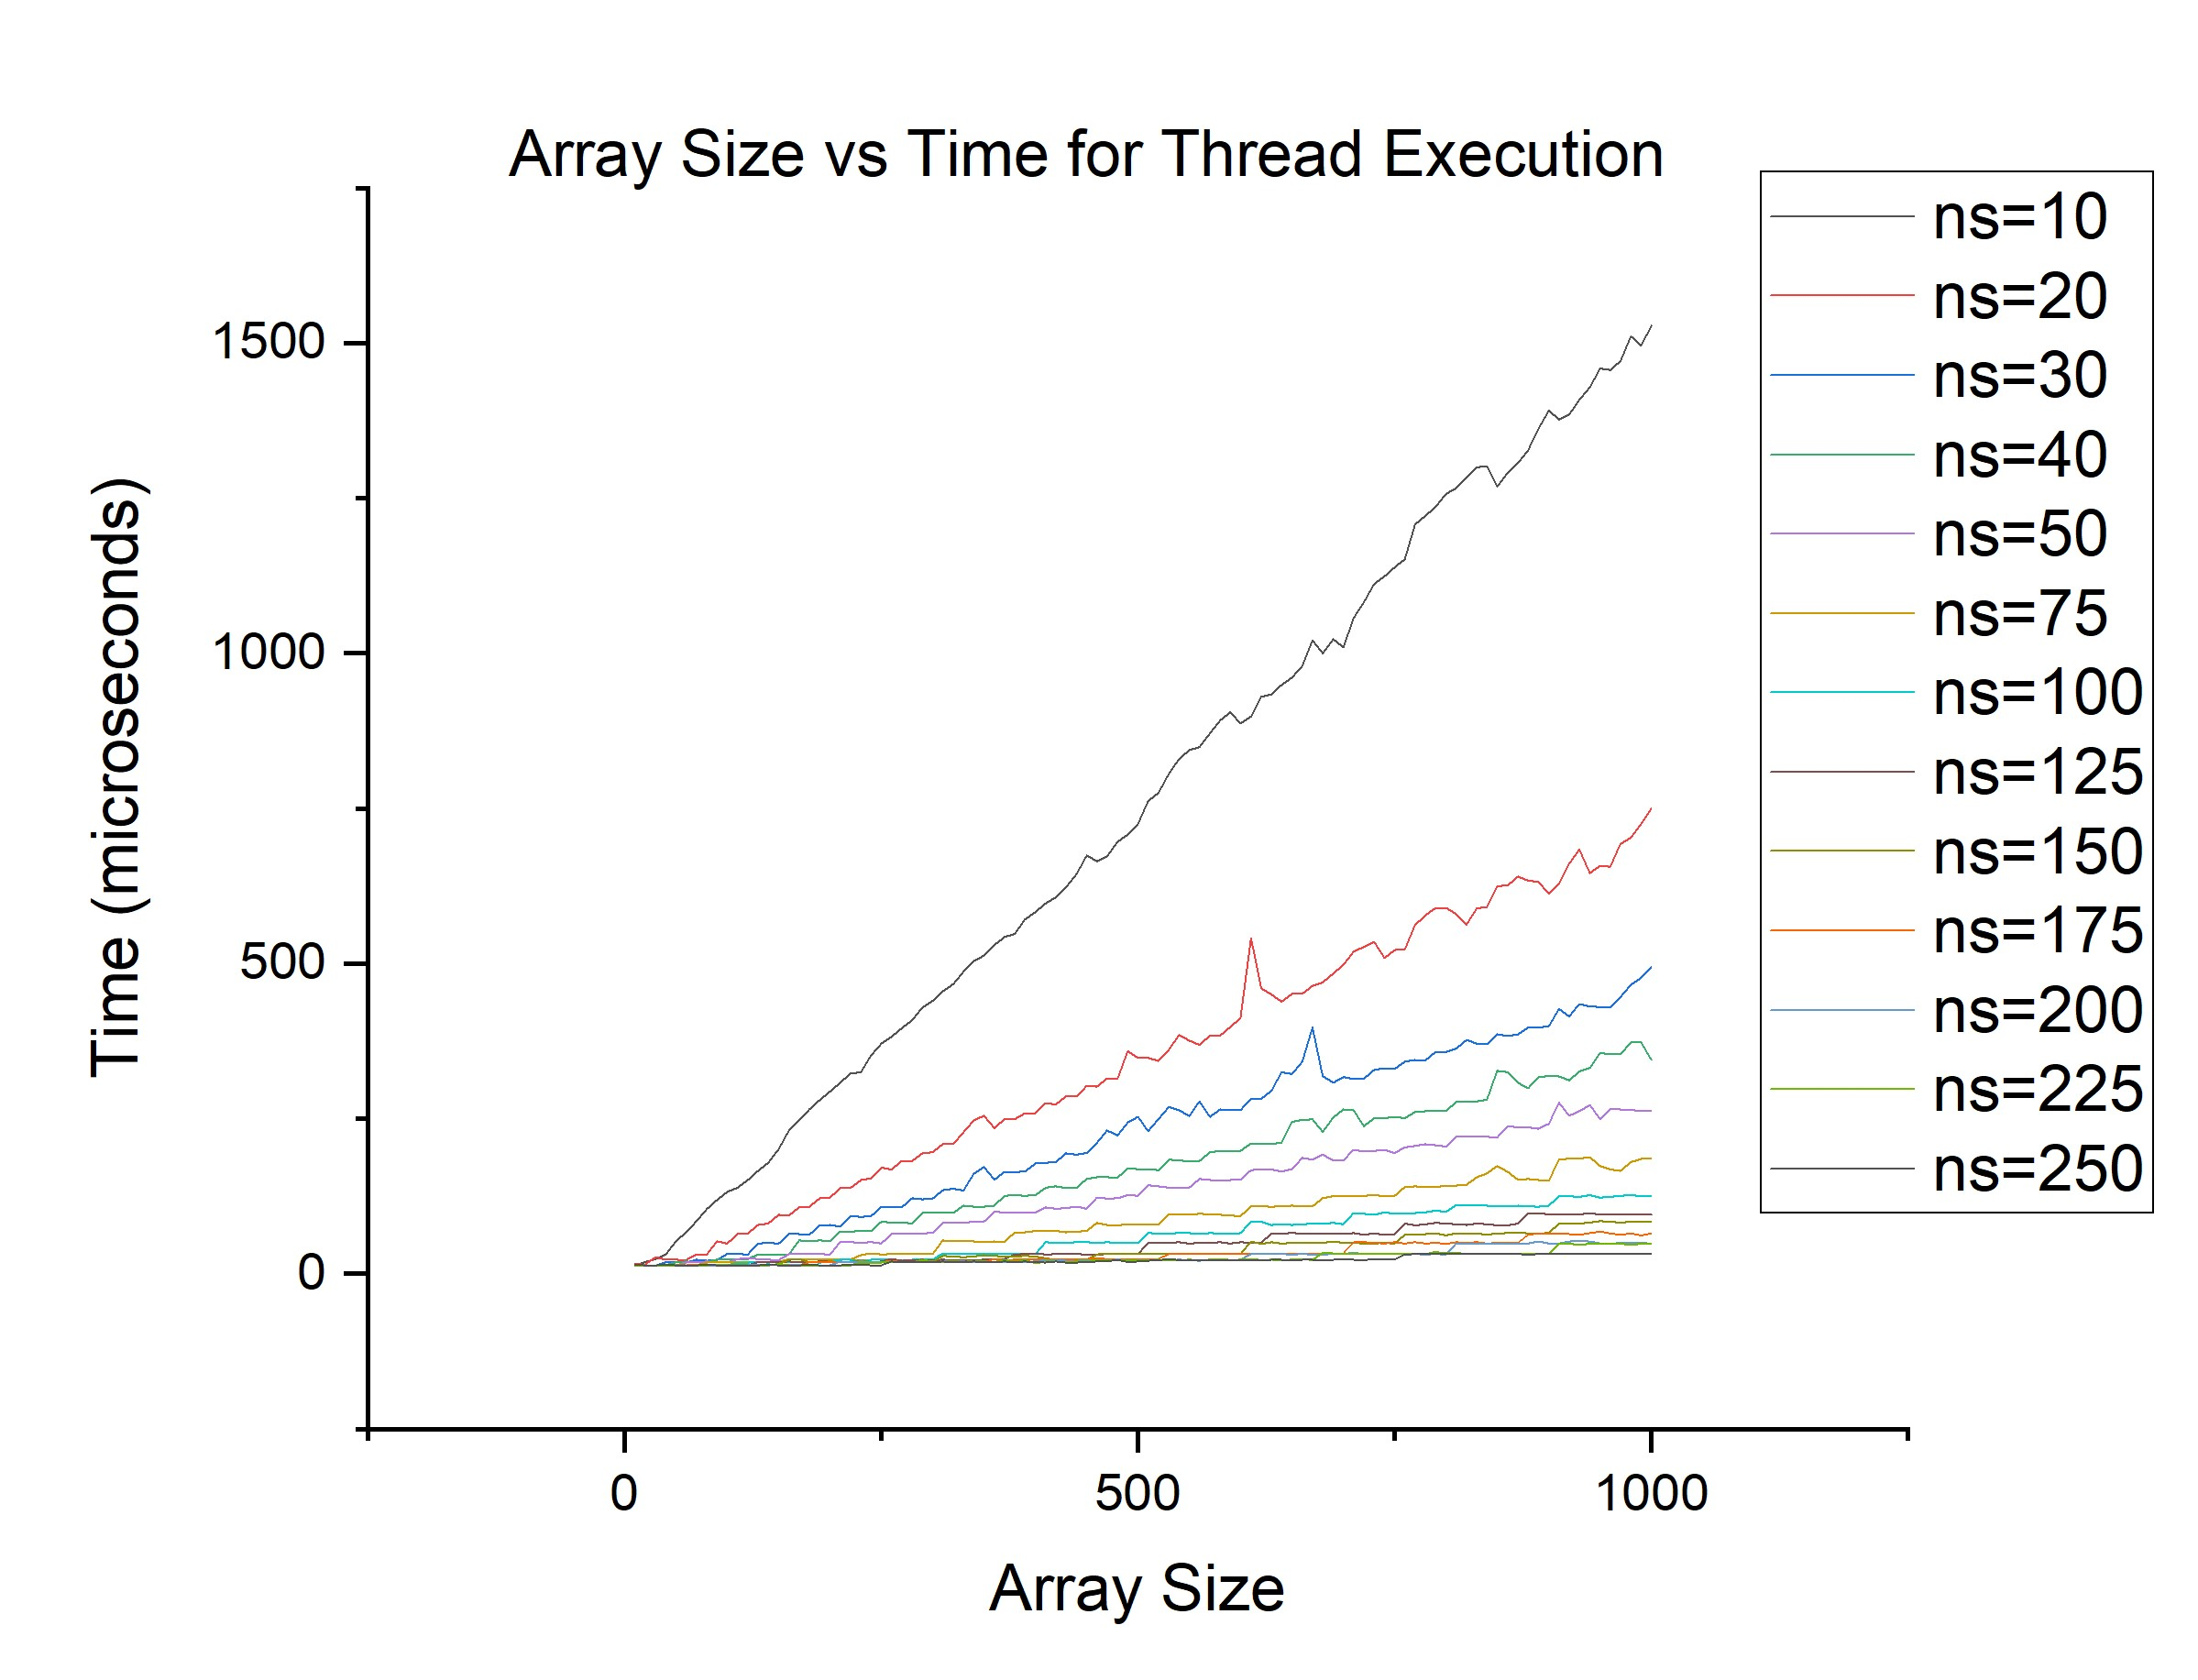
\includegraphics[width=12cm]{svt-Threads}
                \end{figure}
                For \color{red}\textit{Threads}\color{black}, each line represents one case in which the split size(\textbf{ns}) was kept constant.
                It is quite noticeable that as the array size(\textbf{n}) increased, the time increased linearly. 
                This allows us to conclude, with reasonable confidence that, while keeping the number of threads constant, there exists a correlation between array size and time. \newline
                Through our graph, we also can observe a negative correlation between the split size(\textbf{ns}) and the time taken for each execution, but we will delve into that later, as we have data and other graphs available to more clearly illustrate the relationship.
            \subsection*{\color{blue}\textit{\underline{Process:}}\color{black}}
                \begin{figure}[H]
                    \centering
                    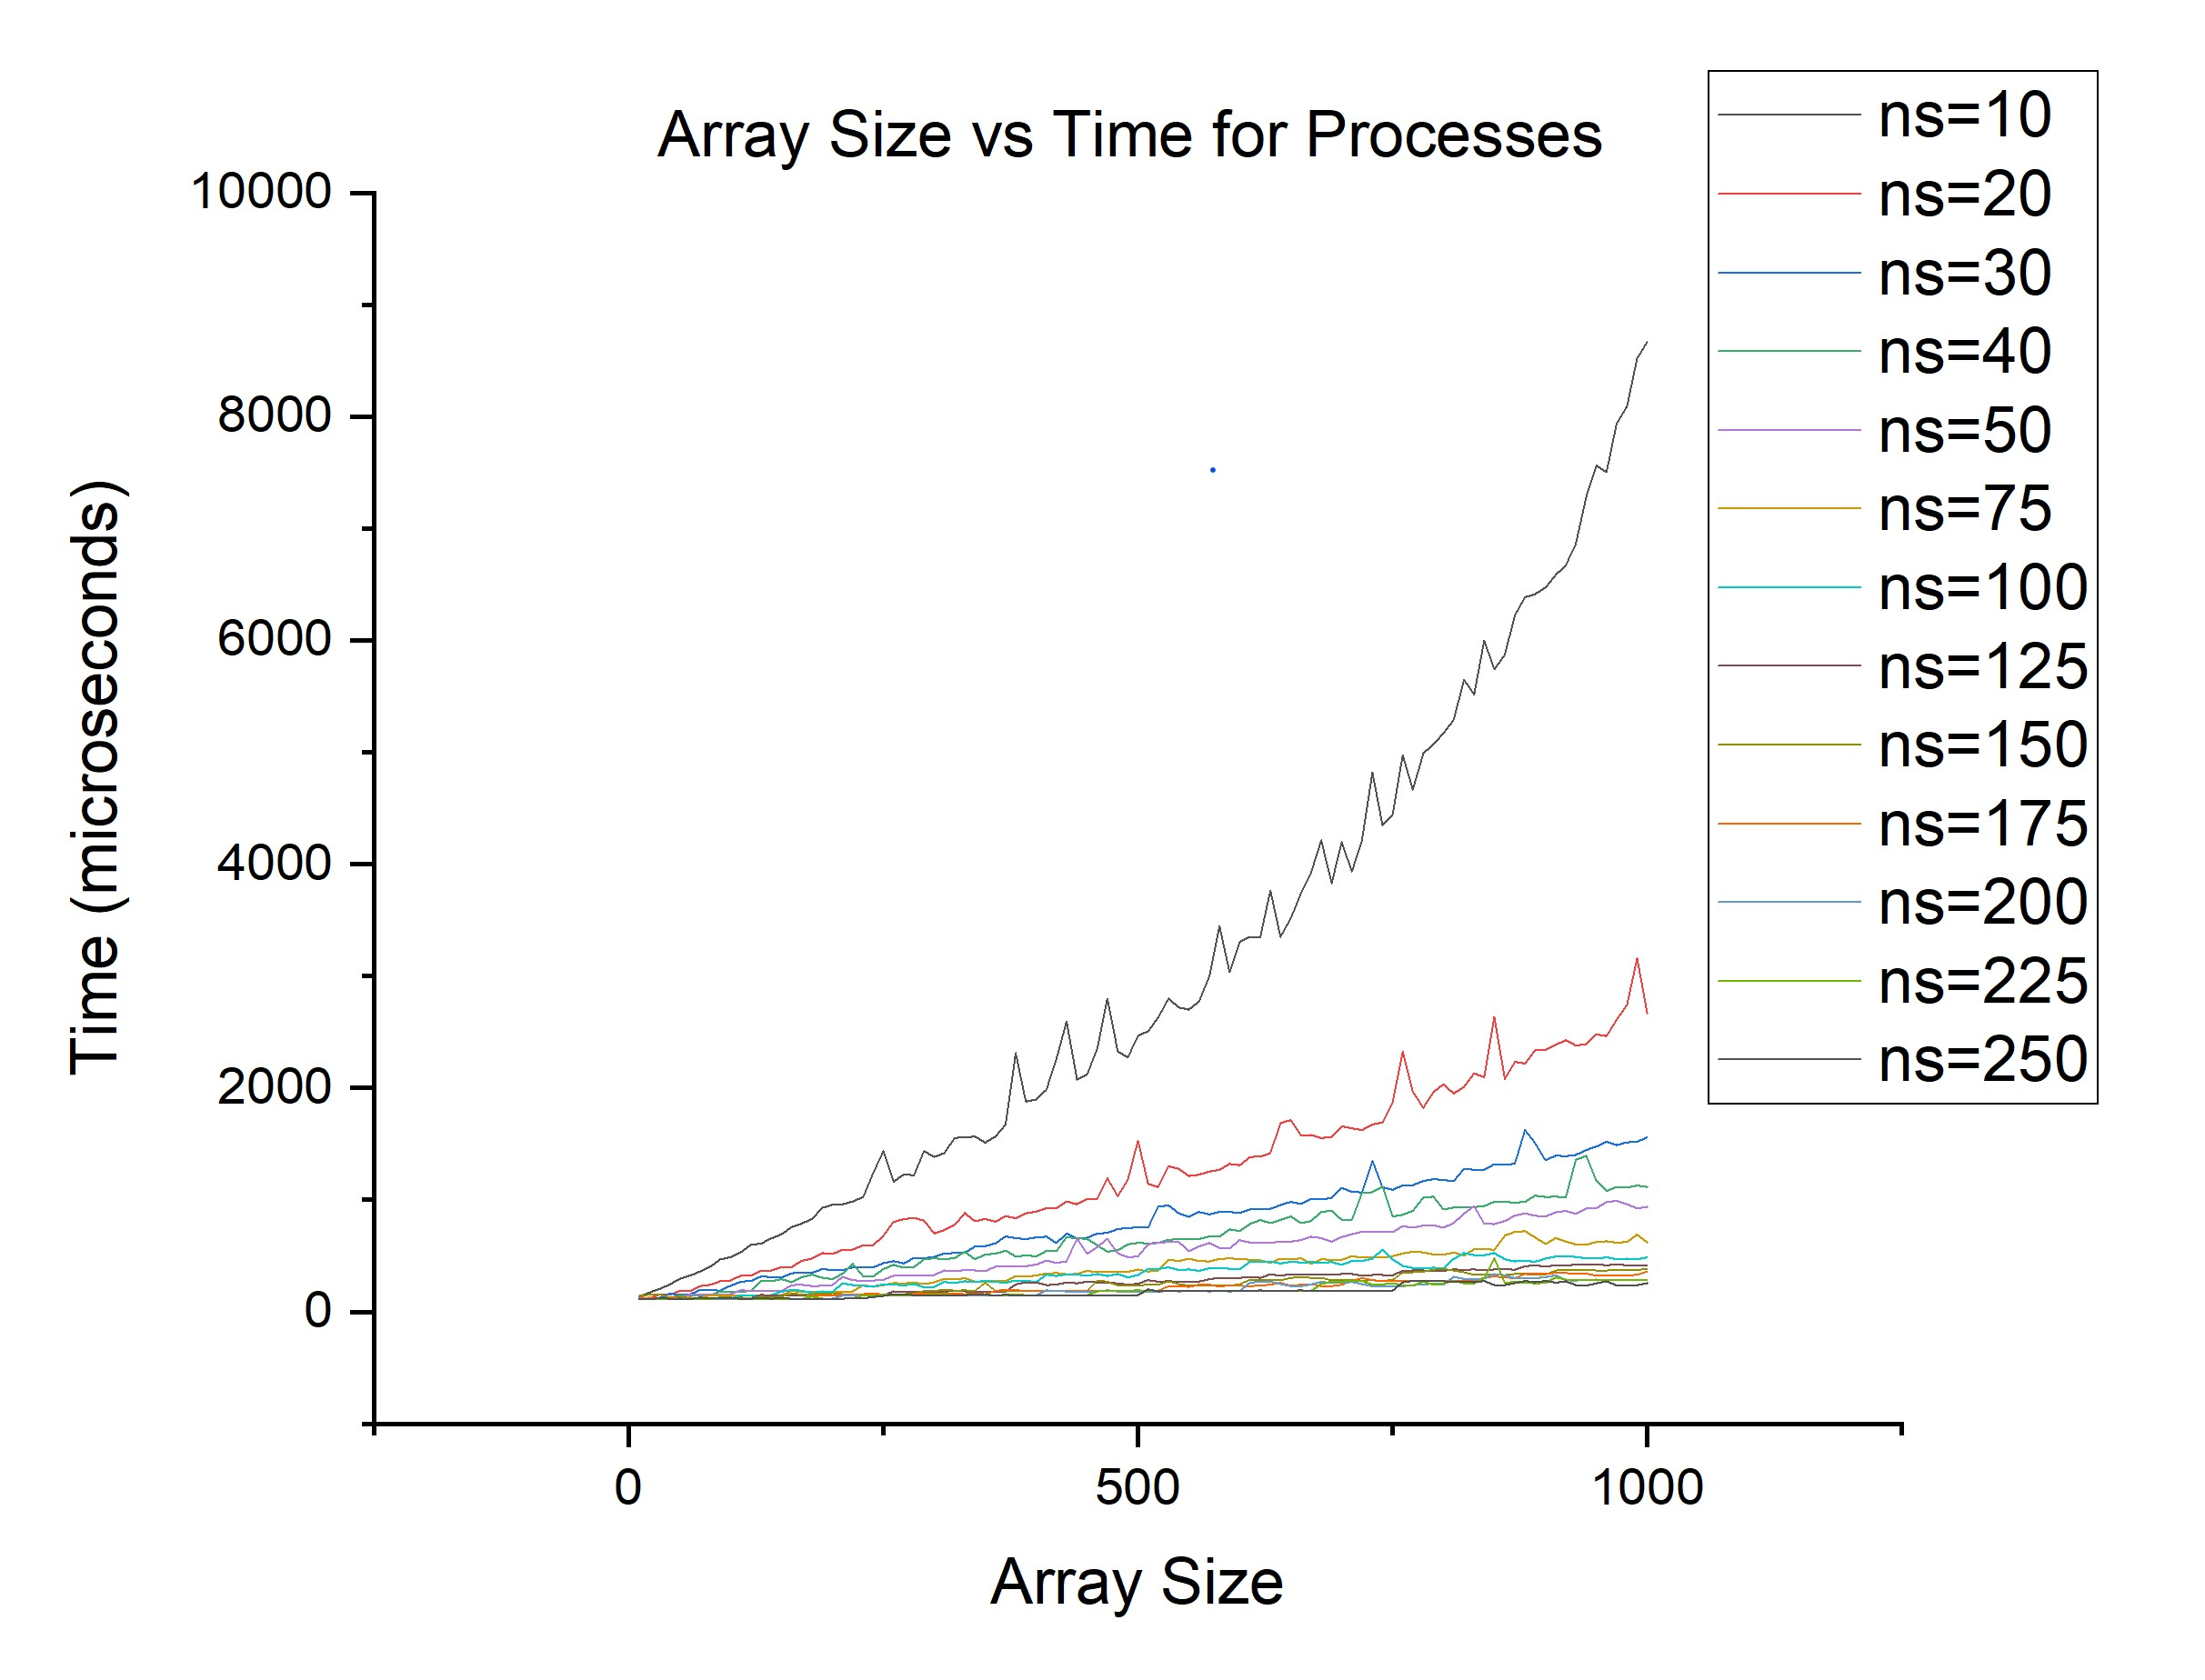
\includegraphics[width=12cm]{svt-Processes}
                \end{figure}
                For \color{blue}\textit{Processes}\color{black}, the graph is very similar to that of \color{red}\textit{Threads}\color{black}. Each line still represents one case in which the split size(\textbf{ns}) was kept constant.
                Similarily to that of \color{red}\textit{Threads}\color{black}, the array size(\textbf{n}) does seem to have an influence on the time.
                However, interestingly, while the split size(\textbf{ns}) is large(i.e. when split size is 250), it is perceived that the graphs are linear. As the split size begins to decrease, we view that the graph is more exponential than linear. \newline
                This seems to be different than what we observed with \color{red}\textit{Threads}\color{black}.
            \pagebreak
            \subsection*{Comparison between \textit{Sequential}, \color{red}\textit{Threads}\color{black}, \color{blue}\textit{Process}\color{black}\ vs. Time}
                \begin{figure}[H]
                    \centering
                    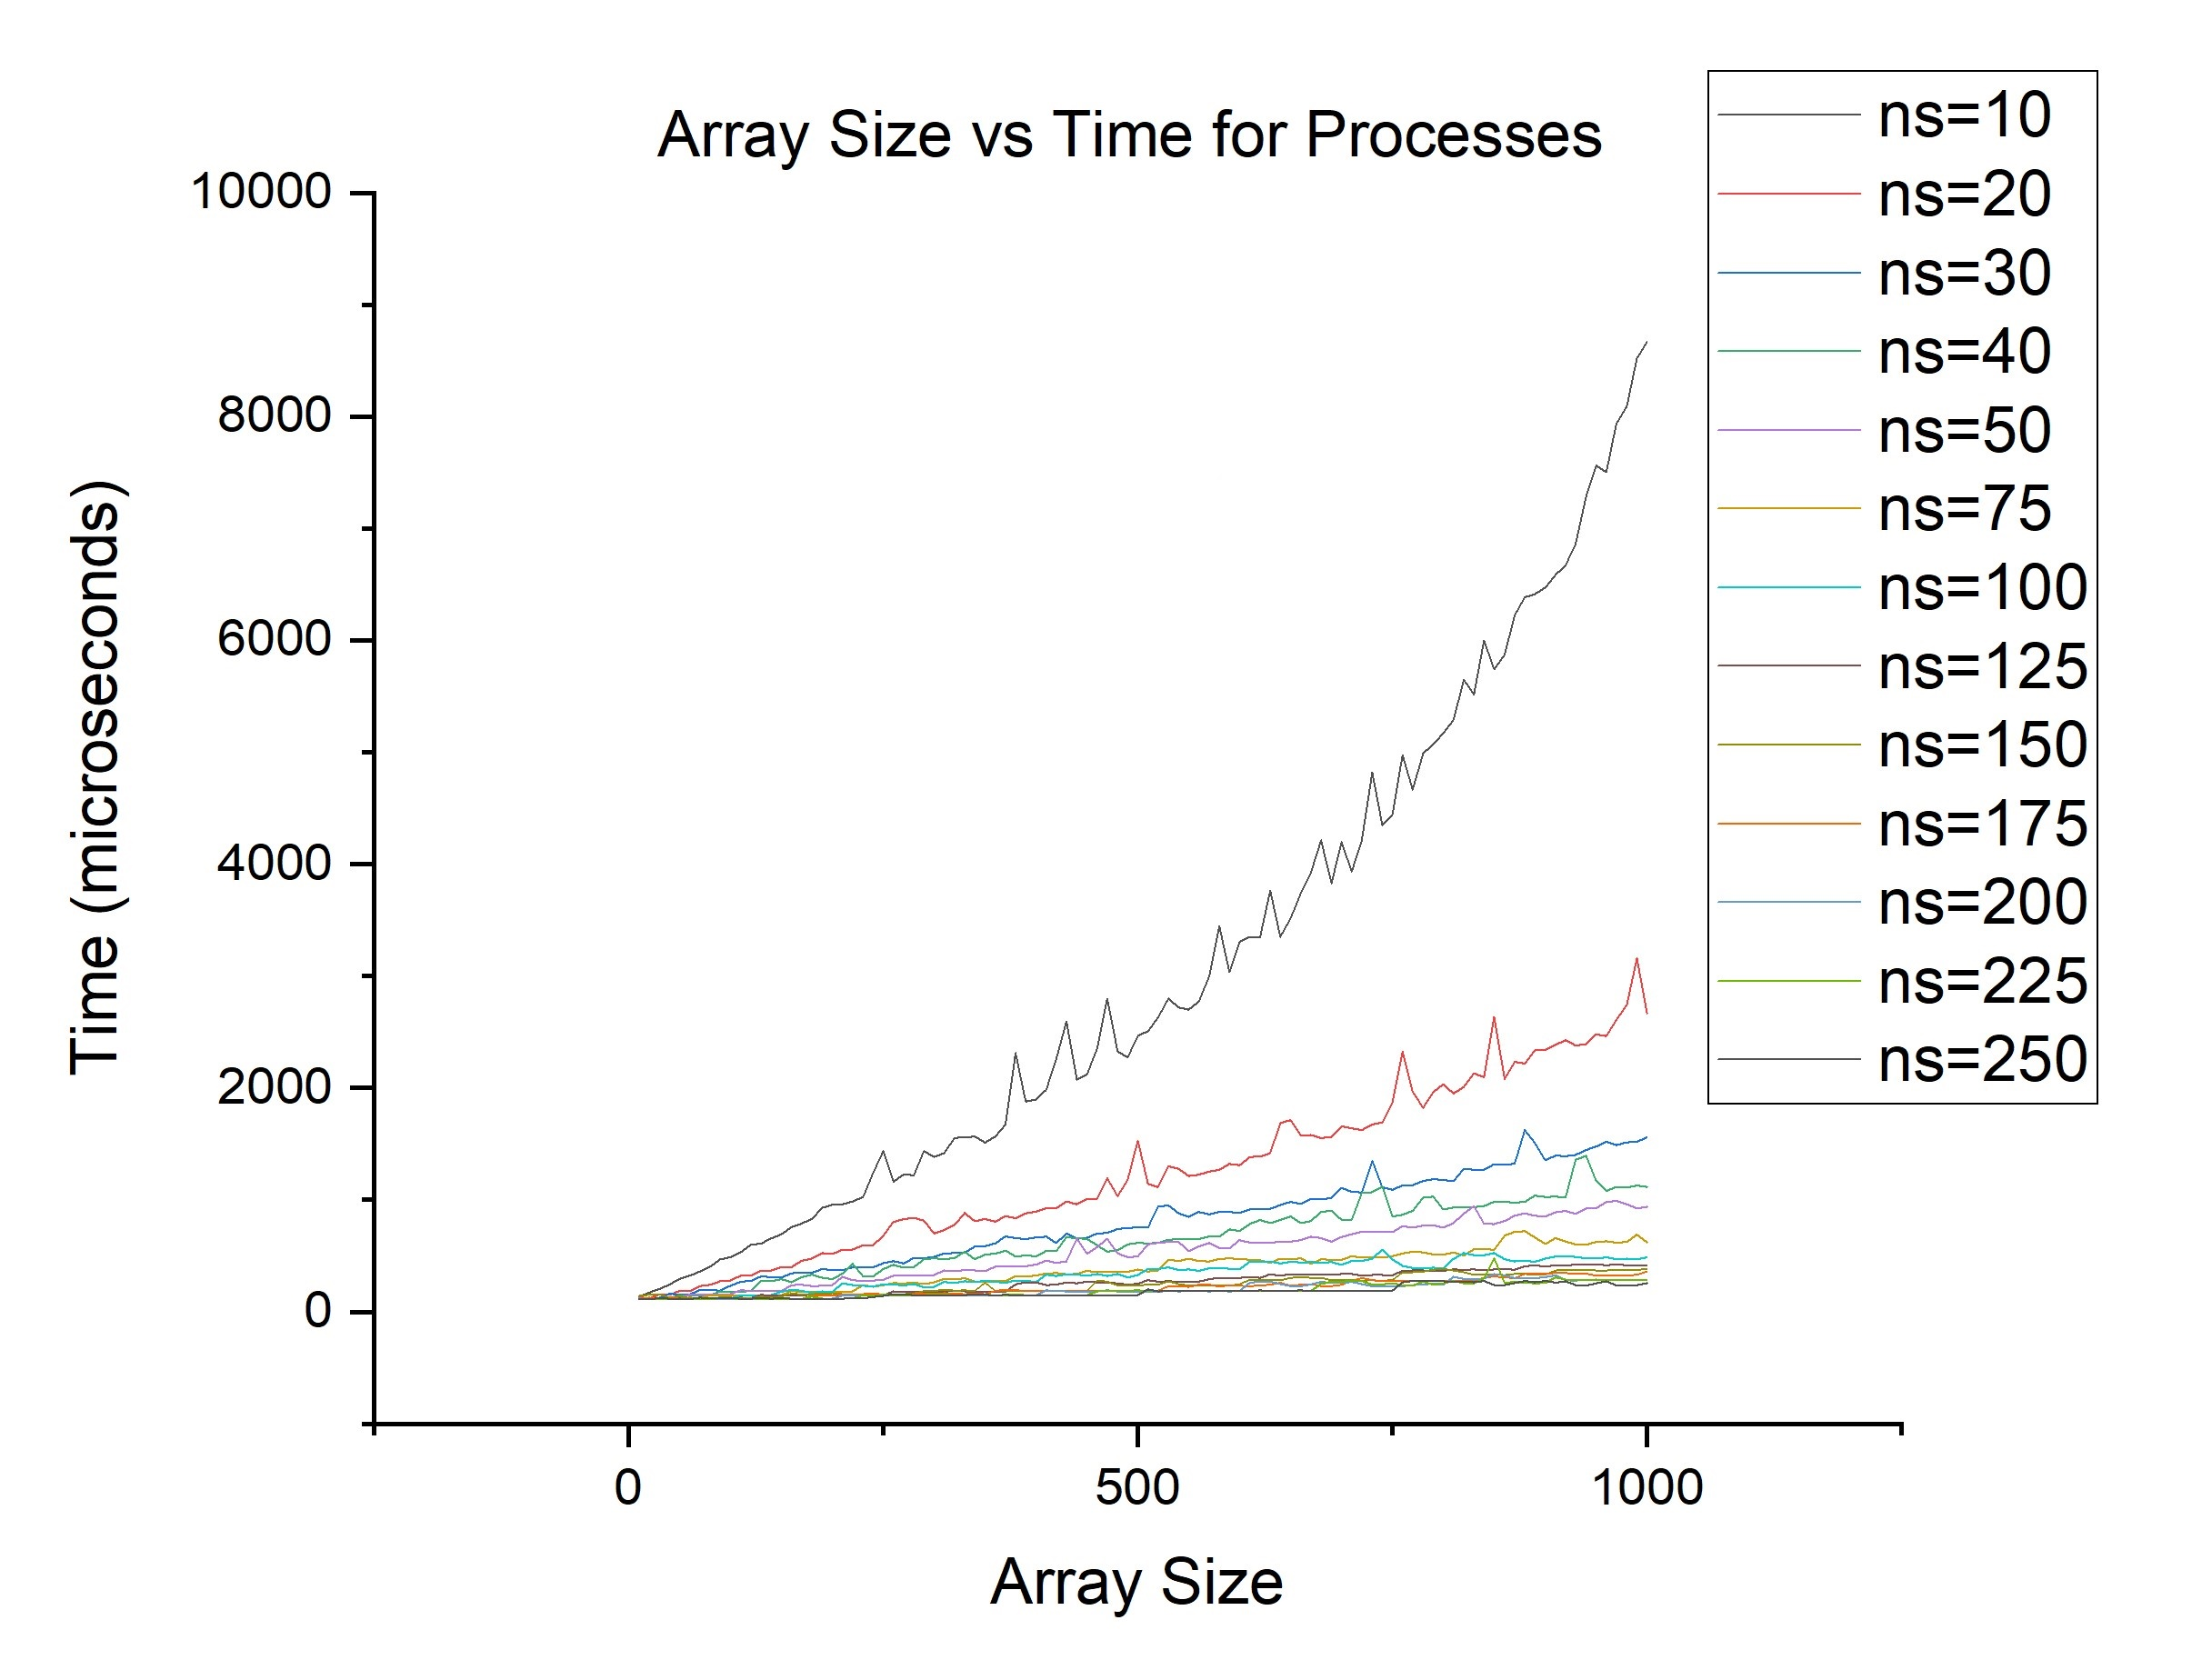
\includegraphics[width=12cm]{svt-comparison-n100}
                \end{figure}
                This graph keeps the split size(\textbf{ns}) constant at a value of 100. 
                Clearly, \textit{Sequential} seems to be almost constant, with the only perturbation occurring as the array size(\textbf{n}) increases to 10,000.
                \color{red}\textit{Threads}\color{black}\ seem to be fairly linear, increasing only a small amount in time per each increase in array size(\textbf{n}).
                \color{blue}\textit{Processes}\color{black}\ seem to be fairly linear as well, but increase time at a much steeper rate than \color{red}\textit{Threads}\color{black}. \newline
                Another important value that we can conclude from this graph is the turning point between using \color{red}\textit{Threads}\color{black}\ and \color{blue}\textit{Processes}\color{black}.
                As shown on the graph, it seems that at 10 threads(\textit{This occurs when array size is 1000 on the graph}) and 1 proccess(\textit{This occurs when the array size is 0-100 on the graph}), the time required for both seem to be similar.
    \section{Conclusion}
\end{document}